\chapter{The Spatial Achromatic Setting (SAPS) Method}
\label{TabletMethodChapter}

\textit{The work presented here has been presented previously as an oral presentation at AIC 2016 \citep[p. 125]{garside_estimating_2016}\footnote{Abstract available: \doi{10.6084/m9.figshare.4269680.v1}} and as a poster presentation at ECVP 2017 \citep[p. 93]{niko_busch_european_2017}\footnote{Poster available: \doi{10.6084/m9.figshare.5478493.v1}}}

\section{Summary}

The principal aim of this piece of work is to explore a novel method for colour constancy experiments, which allows for experiments to be performed in real and complex environments, in order to better understand colour constancy outside of a lab environment. The methodology uses a tablet computer to present a spatial version of an achromatic point setting task. 

The key concerns are whether such a methodology can: a) record differences in perceptual white point, b) present a stable stimulus across disparate environments, and c) be suitable for naive observers following minimal instruction. 

On each point, the method is shown to be at least moderately successful, with caveats, and suggestions are provided for improvements upon the current design. Such a methodology could be used to investigate the effect of multiple cues, conflicting cues and cues which cannot easily be reproduced in a controlled in a lab environment.

\newpage

\section{Introduction}

To further our understanding of colour constancy, investigators have traditionally designed experiments where the number of variables is greatly reduced compared to a real-world environment. This allows investigators to carefully query the impact of any individual variable, or the interplay of a small number of variables. 

For example, a common stimulus-type used in such experiments are `Mondrian' patterns, arrangements of flat and unmoving overlapping coloured paper rectangles, see Figure \ref{fig:mondrian} \citep{hurlbert_colour_1999}. Consider also the experiments of \citet{kraft_mechanisms_1999} where objects representing potential colour constancy cues such as a tin-foil covered cone (specular highlights) were removed from a neutrally coloured box one-by-one in order to probe their relative usefulness (see Figure \ref{fig:KraftBrainard}).

\begin{figure}[hbtp]
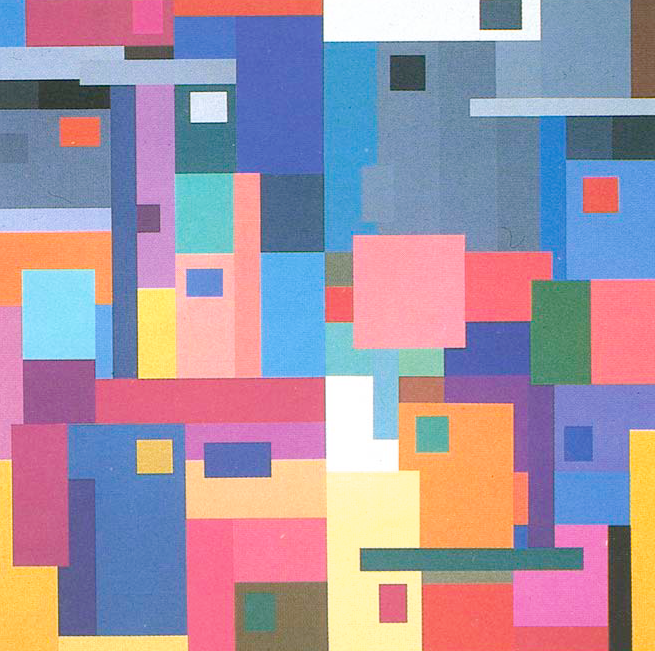
\includegraphics[max width=\textwidth]{figs/tablet/mondrian.png}
\caption{An example `Mondrian', reproduced from \citet{land_recent_1986}.}
\label{fig:mondrian}
\end{figure}

\begin{figure}[hbtp]
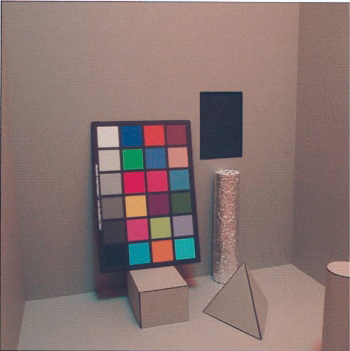
\includegraphics[max width=\textwidth]{figs/tablet/KraftBrainard.png}
\caption{A colour constancy experiment investigating the roles of different potential cues, reproduced from \citet{kraft_mechanisms_1999}. Objects within the scene were carefully selected such that the inclusion or removal or specific objects would allow or exclude the possibility of using a specific mechanism (local adaptation, spatial mean of the image, adaptation to the most intense region) to perform colour constancy.}
\label{fig:KraftBrainard}
\end{figure}

It is clear that these set-ups are much reduced in their complexity compared to a natural scene. Simple experimental stimuli allow for clear questions to be asked, and for those questions to be answered with statistical strength. Such research is valuable. However, the use of simplified stimuli risks overlooking unknown scene attributes, and the human behaviours which may be reliant on them. Experiments often find that colour constancy in lab environments is never `complete'; is this representative of real world behaviour or could this result be due a lab environment failing to deliver all the cues available to an observer in a natural environment? Recent technological advances have enabled experimenters to reproduce natural scenes with increasingly accuracy and comprehensiveness \citep{heasly_rendertoolbox3_2014}, but the number of variables in real scenes is practically infinite, and whilst our ability to reproduce a scene increases over time as technology develops, we only reproduce what we deem important at the time. Using a real-world environment would allow for processes to occur as they do naturally, in the environment for which these processes are presumably optimised (See \citet{kelly_chips_2018} and \citet{shepard_perceptual_1992}.)

There are two clear challenges to the use of natural environments for scientific study; the inability to control target variables, and the influence of uncontrollable or uncontrolled non-target variables. The first challenge may be surmountable; depending on the variable in question it might either be controlled by force, or over time natural variability may provide the required experimental range. The second may be insurmountable but, depending on the specific situation, it may be permissible to consider uncontrolled variations simply as sources of experimental noise. Further challenges arise where connections exist between target and non-target variables, or where the influence of the non-target variables dwarf the effect of the target variable.

One further challenge: it is rare for an experiment in a real-world environment to not intrude onto that real-world scene and change it in some way. The only true solution to this problem would be to consider unannounced observation of a natural behaviour as the only acceptable scientific method. A pragmatic compromise is to design an experiment such that it modifies the environment of the observer minimally, and to carefully consider the impact that the experimental set-up may have upon observers.

The method presented here is a variant of the `achromatic setting' method.\footnote{For overviews see %section X, or 
the section on `achromatic adjustment' in \citet{foster_color_2011} and `Matching to an internal standard' or `achromatic setting' in \citet{smithson_sensory_2005}.} The achromatic setting method requires an observer, under specific conditions, to adjust the chromaticity of an item in their visual field such that this item appears achromatic. Changes in selected achromatic point (in colour space) are thought to represent general adaptive shifts. For example, an observer in an environment lit by a chromatic illuminant would be expected to pick an achromatic point which is shifted towards the chromaticity of the illuminant, compared to the achromatic point which they might select in a more neutral environment. This is often practically achieved by having the `object' be an area of a computer screen, and have it controllable in two or more chromatic dimensions (such as relative amounts of unique red/green and blue/yellow). 

In the \gls{SAPS} method, as presented here, a tablet computer is given to an observer to hold as is comfortable to them, and upon this computer an isoluminant slice through a nominally perceptually uniform colour space is presented, from which they are requested to select (by touching upon the screen with a finger) the point which they deem to be most achromatic (the specific phrase `grey-est or least colourful' is employed in order to make the task suitable for non-colour-scientist observers). The term `spatial' is used since the user provides information by making a spatial selection which directly corresponds to a colour choice, where in other methods abstract sliders or knobs may be used to alter the chromaticity of a static object.

To minimise the effect of the presentation of chromatic scenes upon the viewer, which may influence an observer's state of chromatic adaptation, this process is repeated a number of times with the area of colour space which is presented varying, through random rotation about the luminance axis, and random offsetting through both dimensions of the chromatic plane.

In the rest of this chapter I will describe the method in more detail, and describe some experiments performed to explore the potential abilities and limitations of such a method.

\section{Research Questions and Hypotheses} \label{sec:qandhyp}

\subsection*{Hypothesis 1: The \gls{SAPS} method is suitable for colour constancy experiments}

To be fit for performing colour constancy experiments, this method needs to:

\begin{enumerate}[label=\Alph*.]
    \item \label{list:hyp1a} \emph{Provide a relatively environment-agnostic stimulus.} 
    This experimental method relies on the assumption that the tablet display delivers a stimulus with identical physical properties to the observer independent of environment. In practical terms, this means that the tablet must not be affected by reflection, either at the glossy surface of the tablet display, or at reflection at any other level of the display architecture, to the extent that this has a non-negligible impact upon recorded data. If it is found that this is not the case, the tablet would need to be characterised separately for each environment.
    \item \label{list:hyp1b} \emph{Collect meaningful data.} 
    One would expect this to be indicated by small intra-observer variability (not recording a change where there is presumably none), and reasonable inter-environment change (recording a change where there is presumably a change). It would be expected that these changes would be in line with previously published results.
    \item \label{list:hyp1c} \emph{Additional aim - Be suitable for naive observers.}
    This would reduce the amount of time and effort required to run experiments, and allow for the collection of data from participants less likely to be biased through task expectation. It also means that the demographic group of observers is less likely to be 
    WEIRD (`Western, Educated, Industrialized, Rich, and Democratic', \citep{henrich_weirdest_2010,brookshire_social_2013,justsaysinweird_just_nodate}), white, and undergraduate.
\end{enumerate}

\subsection*{Hypothesis 2: \gls{ipRGC} activation affects perceptual white point.}
Primarily as a proof of concept for this methodology, but also to assist in answering other research questions posed within this thesis, an experiment was performed whereby observers made achromatic selections under a selection of colorimetrically metameric illuminants where there was a melanopic contrast between illuminants. %See section X. 
If \gls{ipRGCs} play a role in colour constancy we would expect to see a distinction between the responses recorded under the different illuminants.

\section{Experimental set-up and methodology}
\subsection{Method \& Apparatus}

\subsubsection{Instructions to the participants}

The observer was instructed to hold the tablet such as was comfortable for them to do so, upon which the first trial of the experiment was already visible. They were instructed to `touch the grey-est, or least colourful, point on the screen'. Upon touching the screen, the stimulus would be replaced with a new stimulus. This new stimulus was a new subsection of the full stimulus image (See Figure \ref{fig:Stimulus}) which had been randomly rotated and offset (further information provided in Section \ref{sec:stimuli}).

Most observers seemed to find this task difficult for the first stimulus, but within the first few stimuli seemed to develop an increased comfort and ease with the task, which resulted in a decreased response time. %(Illustrate with graph of response time?)
At this point the observer was told that there would be thirty trials. No training was provided, and no runs were excluded as training runs. One stimulus was forced to have identical rotation and offset to an earlier stimulus, in order to assess intra-observer variation (see Section \ref{sec:exclusion}).

\begin{figure}[hbp]
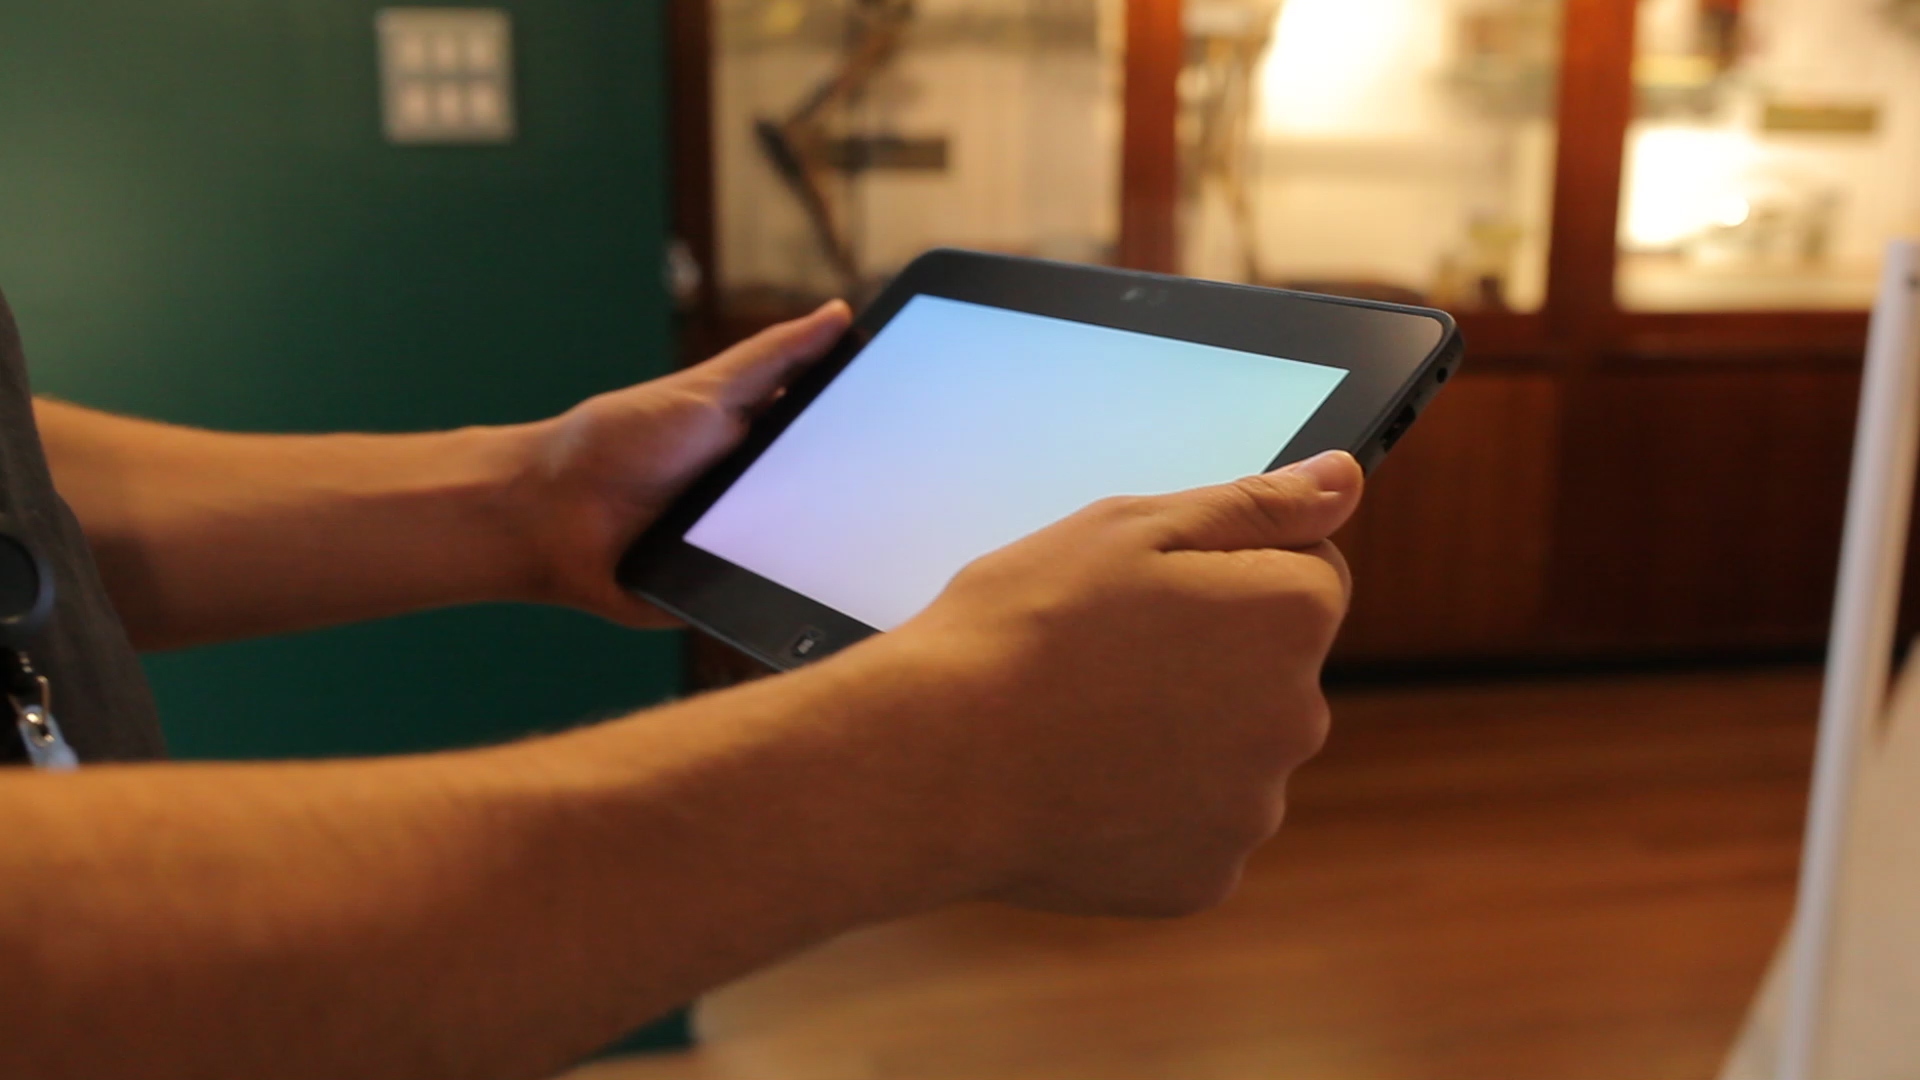
\includegraphics[max width=\textwidth]{figs/tablet/MVI_3213-1.jpg} % E:\Pictures\2016\2016-10-14
\caption{A participant (the author) holding the tablet with a stimulus on screen.}
\label{fig:grant_demo}
\end{figure}

\begin{figure}[hbp]
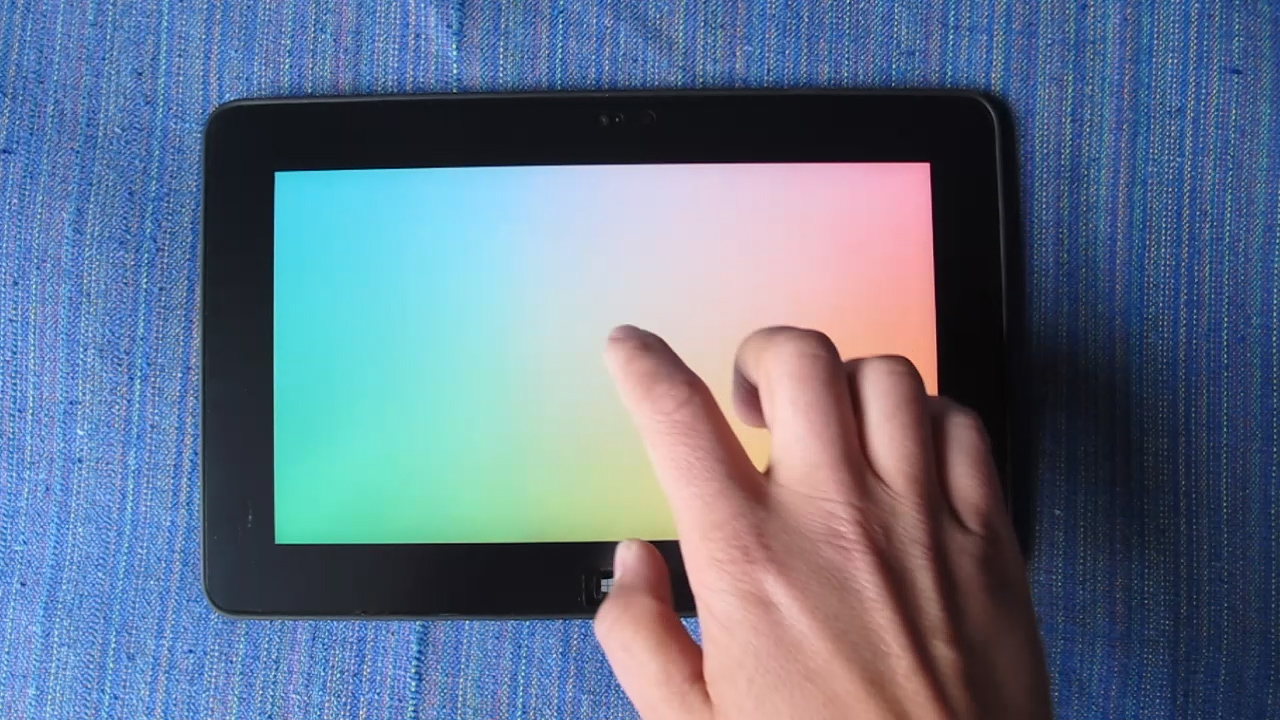
\includegraphics[max width=\textwidth]{figs/tablet/MVI_3889-4.jpg} % E:\Pictures\2016\2016-10-18
\caption{A stimulus displayed upon tablet and finger in motion towards subjective point of achromacy.}
\label{fig:finger}
\end{figure}

Following the thirty trials, a secondary task was presented to observers, designed to characterise their touch input. This task features a 2x2 checker board pattern upon a black background (See Figure \ref{fig:checker-board}). Observers were instructed to touch the centre of this checker board. Upon registering a touch, a new checker-board would be presented, of the same attributes but modulated in position in the same way as the main stimulus. This data was later used to calibrate touch input, and to ascertain the amount of measurement uncertainty derived from touch input. 

\begin{figure}[hbp]
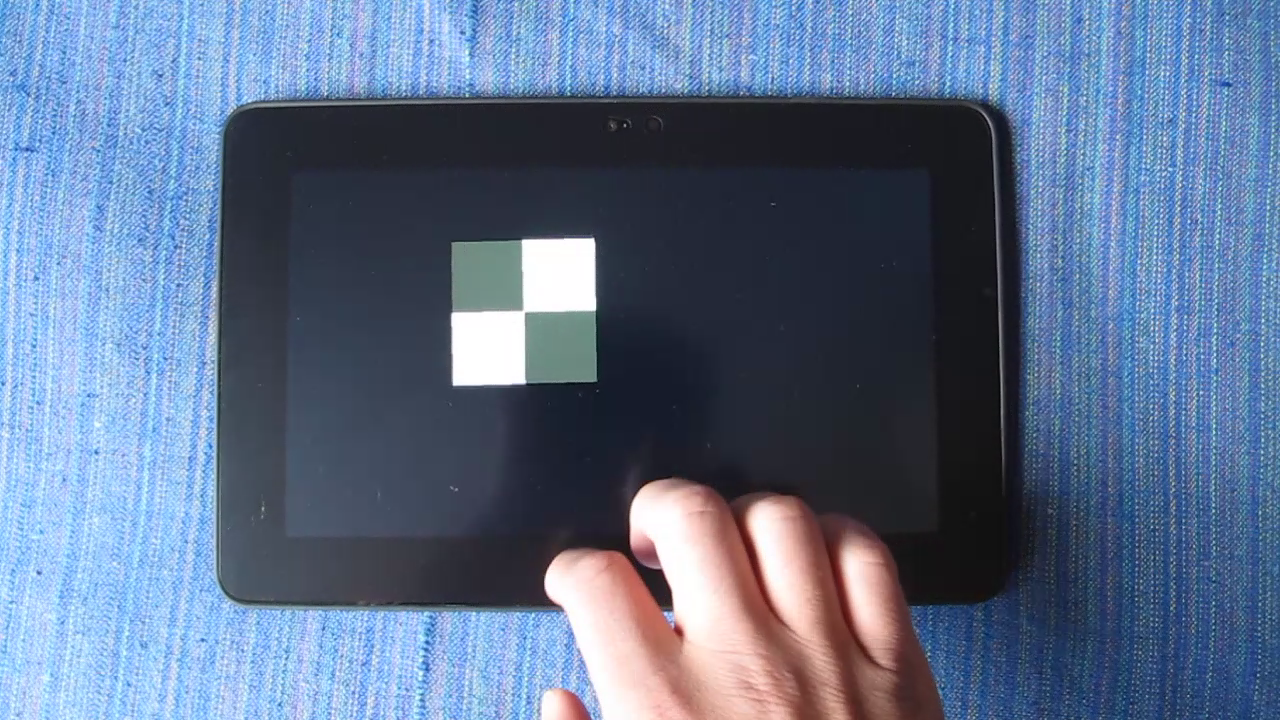
\includegraphics[max width=\textwidth]{figs/tablet/checker_board.png} % E:\Pictures\2016\2016-10-18
\caption{Photo of checker-board task. Participant is requested to touch centre of the checker-board pattern.}
\label{fig:checker-board}
\end{figure}

%Doing this without incentive for participants meant that it was rushed (?)

\subsubsection{Specification of tablet PC}

Participants undertook the experiment upon a Dell Latitude 10 ST2 tablet computer with `BROTECT' Matte Screen Protector (223x126mm active screen area, 1366x768 pixels). This tablet was chosen for its ability to run a Windows environment, and the matte screen protector was added to reduce the severity of specular reflections. The measured gamut of this device is shown in Figure \ref{fig:gamut}.

\begin{figure}[hbp]
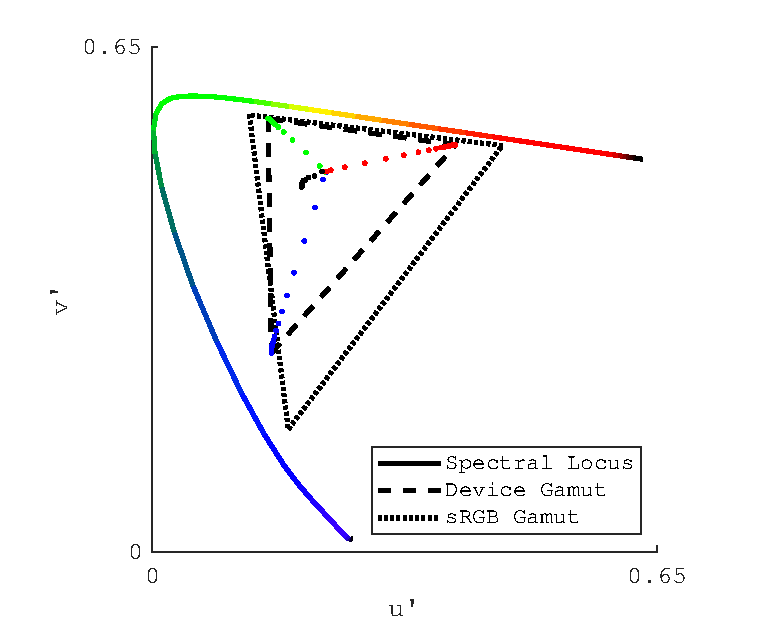
\includegraphics[max width=\textwidth]{figs/tablet/gamut.pdf}
\caption{The display gamut. Red, green and blue dots indicate chromaticities of single channels at different pixel values. The black dots are the chromaticities achieved when the pixel values are kept in line for each channel. This can be described as the native white point of the display.}
\label{fig:gamut}
\end{figure}
% Generated using the 'Plot gamut' section of SAPS_TabletCharacterisation.m

\subsubsection{Selection of colour space for creating the stimuli}

The stimulus presented to observers was an isoluminant plane (in CIE L*) through CIELUV colour space. CIELUV was chosen for having an associated object colour space, where comparisons between the chromaticity of light sources and the chromaticity of selections could be made. 

\subsection{Stimuli} \label{sec:stimuli}
\subsubsection{Generating the stimuli}

The stimulus was specified as: L*: 60 uniformly across field, u*: ranging linearly from -50 to 50 from one side of the field to the other, and v*: as for u*, but along the orthogonal axis, so that the stimulus was of uniform lightness and smoothly changing hue and chroma. The full stimulus image (Figure \ref{fig:Stimulus}) was 2188 pixels square; this is larger than the pixel dimensions of the screen to allow for the stimulus to be rotated freely and offset by up to a third of the image in any direction before the edge of the image is encountered. 

The stimulus was specified with the above attributes in a matrix within MATLAB\footnote{Code: \url{https://github.com/da5nsy/SAPS/blob/21940bb6ed9d0e37d88e1b655f4919d73431743a/experiment/stimulusGenerator002.m}}. CIELUV values were converted to XYZ tristimulus values using built in functions, with reference white set as the XYZ tristimulus values of the display at maximum white (with screen protector), as measured with an Xrite i1 device. Linearisation was achieved through the use of a look-up table, computed by spline interpolation of the measured outputs at 15 pixel %(KT: pixel drive value?)
value increments from 0 to 255 for each channel. The stimulus was then output as an 8-bit tiff image, which could be easily loaded and manipulated by the psychophysical stimulus presentation software PsychoPy \citep{peirce_psychopypsychophysics_2007}. %(Illustrate with flow diagram?)

\begin{figure}[hbp]

\includegraphics[max width=\textwidth]{figs/tablet/stimulus.png}
\caption{Full stimulus image.}
\label{fig:Stimulus}
\end{figure}
% Copied and pasted from original psychopy folder. Could regenerate using stimulusGenerator002.m

\subsubsection{Presenting the stimuli}
A program was written in PsychoPy\footnote{\url{Code:  https://github.com/da5nsy/SAPS/blob/21940bb6ed9d0e37d88e1b655f4919d73431743a/experiment/SpatialAchromaticPointSetting_0940_Grant.py}} that presents the stimulus 30 times, with random rotation and random offset in the horizontal and vertical dimensions of between -1/6 and +1/6 of the respective dimension. Thus `objective grey', where [u*,v*] = (0,0), was always within the central third (in each dimension) of the screen. This program saved details of the stimulsu offset and rotation (`dpX', `dpY' and `ori'), co-ordinates of observer selected point (`x-co\_raw', `y-co\_raw', and also `direction\_raw', `magnitude\_raw'), and time taken to make selection, measured since last selection (`toc\_raw').

The effect of rotation and offset was that on each stimulus presentation the observer saw a stimulus that appeared somewhat different to the previous stimulus, but still hopefully included their preferred achromatic point. The rotation and offset can be illustrated by plotting the chromaticities present in any one stimulus presentation, as in figure X. %!!!!!!!!!!!!!!!!!!!
Plotting the chromaticities present across a full run of 30 trials yields Figure \ref{fig:practical}, where it can be seen that the rotation results in a roughly circular spread of chromaticities, and the rotation and the offsetting together result in a gradient of likelihood of presentation which is high at the centre of the full stimulus and lowest at the edges of the full stimulus. This gamut distribution is referred to further in the text as the `practical gamut'.

% Single shot figure needed

% \begin{figure}[hbp]
% \includegraphics[max width=\textwidth]{figs/tablet/????}
% \caption{A representation of the chromaticities present in a single stimulus. Note that the gamut is not rectangular for 2 reasons: firstly, because CIELUV is not a linear transformation of CIE u'v' , and secondly because for this particular stimulus, the bottom left corner (as presented above) intersects with the display gamut boundary, resulting in a gamut compression to that corner.}
% \label{fig:?????}
% \end{figure}


\begin{figure}[hbp]
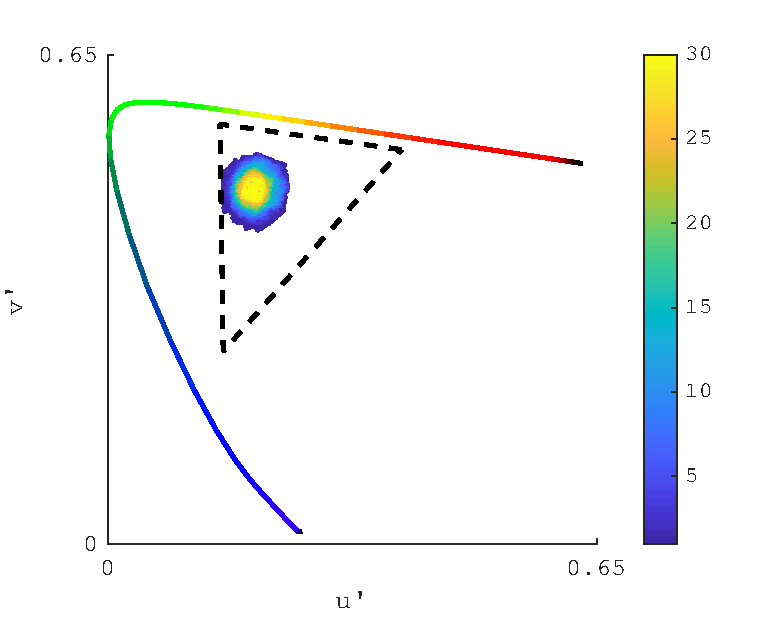
\includegraphics[max width=\textwidth]{figs/tablet/practical_gamut.pdf}
\caption{The `practical gamut'. This plot shows the relative frequency that chromaticities are actually presented, within the boundary of the device gamut (as shown in Figure \ref{fig:gamut}). The highest number of times a particular chromaticity can be presented is 30, since there are 30 trials in a typical run. As described in the main text, chromaticities falling towards the specified objective white point of the stimulus are presented every stimulus, whereas those further away from the centre of the stimulus are presented less frequently. On the left-hand side of the cluster it can be seen that the gamut boundary is reached. This is discussed further in section X. %!!!!!!!!!!!
}
\label{fig:practical}
\end{figure}


\subsubsection{Touch input characterization} \label{sec:touch}
The checker-board stimuli (Figure \ref{fig:checker-board}), included to allow for fine spatial calibration for individual observers' touch input, was generated by running the main experimental script again but with the stimulus file path replaced with a simple pattern generated within PsychoPy.

I hypothesize that any shifts in touch input would be the result of one or both of two potential influences: `fat fingers' and hardware calibration. By the former I refer to the fact that whilst a finger is considered to be a relatively discrete unit, controlled with presumed dexterity and accuracy, the specific part of the finger which touches the screen will vary from person to person. By the latter I refer to the fact that it is highly possible for there to be a `fairground gun effect', whereby the hardware introduces a reliable bias due to calibration misalignment.

\subsubsection{Limitations of the stimuli}

\subsection{Environments}

\subsubsection{\gls{UCL} Grant Museum of Zoology}

The \gls{UCL} Grant Museum of Zoology is a natural history museum within \gls{UCL} with over 68,000 specimens, which is open to the public and also used as a teaching resource. It is lit with a mixture of daylight and \gls{LED} lighting, and a rarely used fluorescent lighting system (not used during any experiments).
This space was used for preliminary experiments. 

\begin{figure}[htb!]
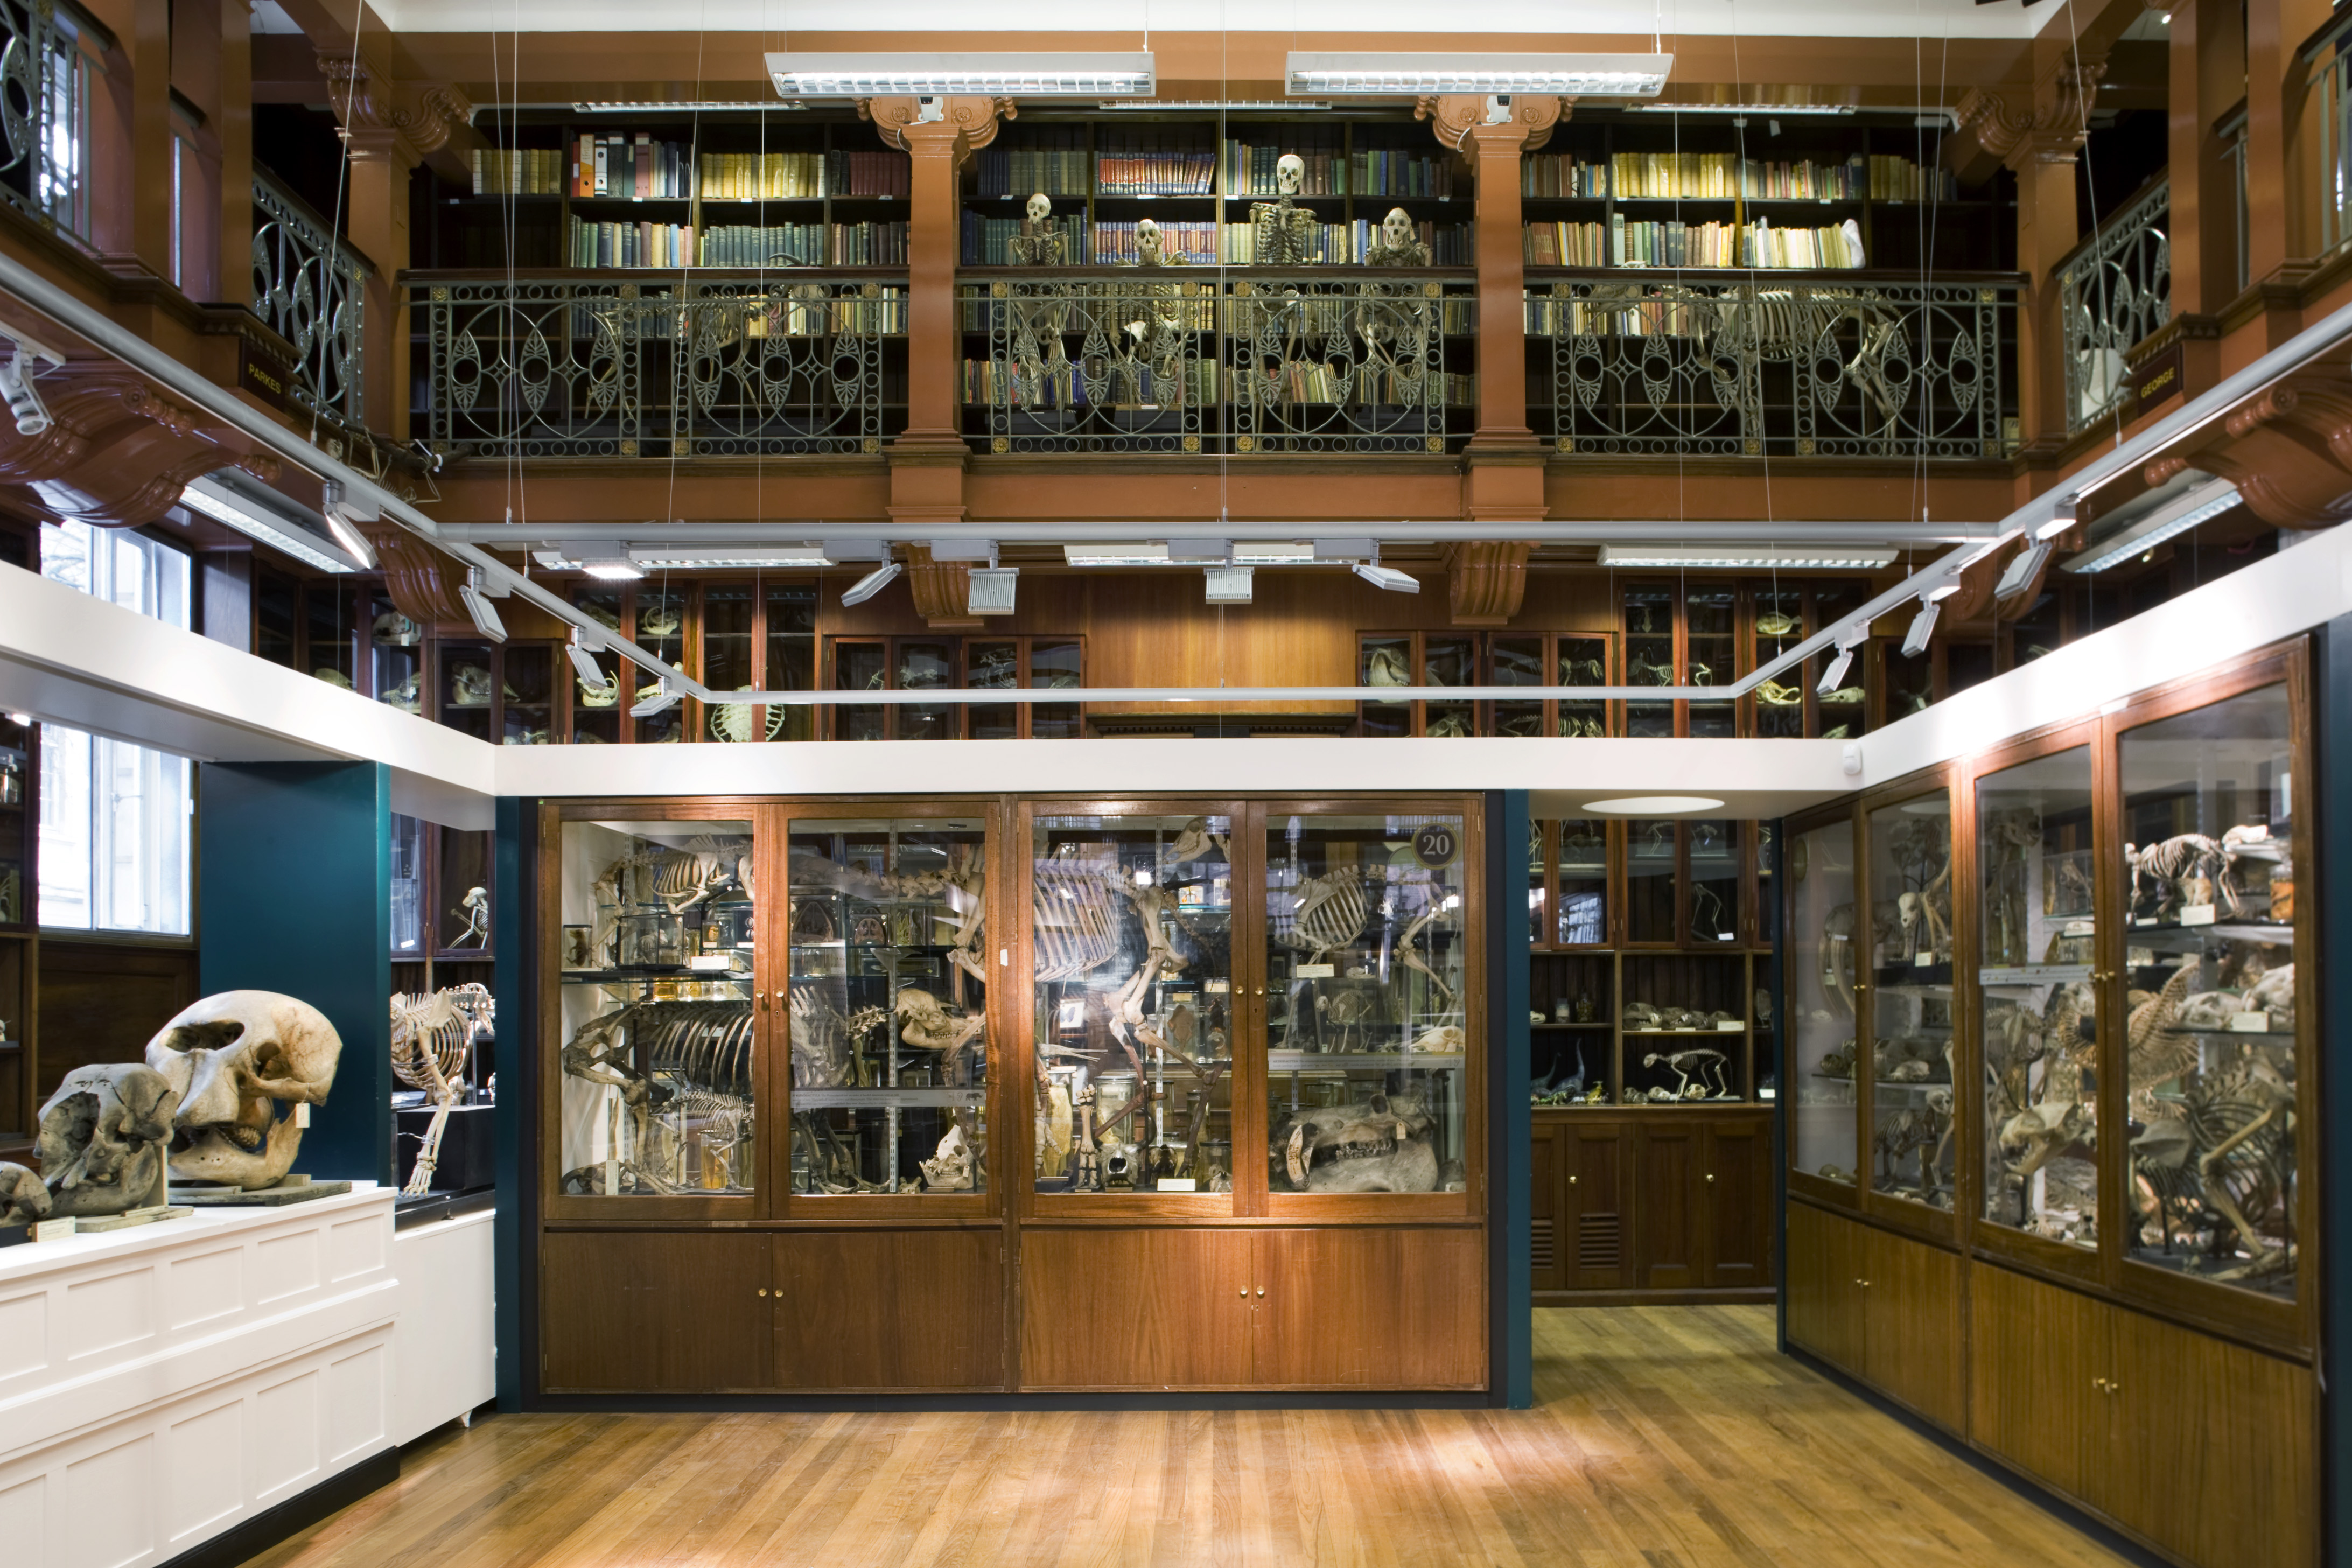
\includegraphics[max width=\textwidth]{figs/tablet/grant.jpg} 
\caption{The central space at the \gls{UCL} Grant Museum of Zoology. Note the daylight on the left, the \gls{LED} lighting at mid-height and the fluorescent lighting at the very top of the image. Image copyright: \gls{UCL} and Matt Clayton.}
\label{fig:grant}
\end{figure}

\subsubsection{The British Museum} \label{sec:BM}

The British Museum is a large museum located close to the main \gls{UCL} campus, which exhibits artefacts of artistic, cultural and historical relevance. 

Three spaces within the museum were used (with permission):

\begin{itemize}
    \item Rooms 77/78 (`Greek and Roman Architecture', `Classical Inscriptions'), lit with fluorescent lighting.
    \item Room 25 (`Africa' - specifically the east section of the room), lit with tungsten  lighting.
    \item The Queen Elizabeth II Great Court (referred to as `GC'), lit with filtered daylight \citep{foster_and_partners_london._great_2002} during daylight hours, with additional lighting at twilight and after sunset. All experiments were carried out during daylight hours, where additional artificial lighting was not employed.
\end{itemize}

% Photos of spaces
% BM SPD figure

\subsubsection{\gls{PAMELA}} \label{sec:PAMELA}

\gls{UCL} \gls{PAMELA} consists of a large open space, enclosed within a light-proof warehouse, and is most often used for its customizable floor space, where small sections can be independently raised or lowered to recreate the spatial configurations of public spaces such as streets or railway platforms. It is of interest to this project since it also has a customizable lighting rig comprising 44 addressable fixtures, each with 6 independent channels, which is controlled via a PC interface. There is an additional high power white channel, which is on a separate control system. 

% Photo(s) of space
% PAMELA screenshot

For experiments reported here three illumination settings were defined - `Cool White (`CW')', `Warm White (`WW')', and `Mel-High (`MH')'. `CW' and `WW' were system defaults, and `MH' was defined to be a colorimetric match (for the CIE 1931 observer) for `CW', but preferentially using an \gls{LED} band with a peak spectrally close to the peak spectral sensitivity of melanopsin (~480nm).

It should be noted that luminance was not matched between the conditions. Therefore, `CW' and `MH' could be described as colorimetric matches, but not as metameric matches. Additionally, for chromatically distinct conditions (`CW' vs `WW'), there is a confound of luminance variation. The luminances of the three conditions were 235lx, 720lx and 840lx respectively. In the opinion of the author, it would be advisable that if further studies of this type were undertaken, that conditions be matched for luminance in order to discount this as a variable. 

% SPD plots of CW, WW, and MH

The chromaticities of the light sources, measured with a UPRtek MK350, were:
`WW': 	u'v'(0.248,0.524) (averaged over 4 measurements)
`CW': 	u'v'(0.200,0.465) (averaged over 3 measurements)
`MH': 	u'v'(0.201,0.467) (averaged over 8 measurements)
The chromaticity co-ordinates of `CW' and `MH' are close enough to be considered as colorimetrically matched for the CIE 1931 standard observer. %who says?

% colorimetry plots

\subsubsection{\gls{UCL} Chadwick Building}

Additional testing was undertaken within the Chadwick Building of \gls{UCL} (home of the Department of Civil, Environmental and Geomatic Engineering), in light-tight basement rooms fitted with fluorescent lighting.

\subsection{Participants}

For studies conducted at The British Museum and The Grant Museum of Zoology, observers were selected randomly from visitors. A visitor would be approached by the experimenter (DG) and asked whether `they would be interested in taking part in a colour vision experiment'. Those who replied positively were verbally informed of the ethics details for the study, the principal parts of which were: that no identifying information would be recorded, that the experiment carried no risks greater than those associated with normal use of a tablet computer, that observers were not paid or otherwise incentivised to take part, and that the task would take roughly ten minutes. This study was approved by the \gls{UCL} Ethics committee: Project ID Number: 9357/001. %[Appendix X] !!!!!!!!!!!!!

For trials at `\gls{UCL} \gls{PAMELA}', participants were recruited from the author's friends and family, with the hope that this would assure attendance and motivation and to take advantage of short-notice availability of the experimental space. Participants were informed of the ethics details for the study in advance of attending. Ethics approval was provided following the amendment of the aforementioned ethics application (9357/001).

\subsection{Data Analysis}
\subsubsection{Processing Pipeline}

The data was analysed in MATLAB using the following pipeline:
\begin{enumerate}
\item Data loaded into MATLAB from an excel file
\item Spatial touch points calibrated using touch characterization data
\item Spatial data converted into chromaticity data
\item Data graded for performance and exclusions applied where appropriate (see Section \ref{sec:exclusion} for further details) 
\item Data plotted either as:
\begin{enumerate}
\item Full dataset scatter
\item Standard deviation ellipse/line plotting\footnote{Based on code from: \url{https://stackoverflow.com/a/3419973}}.
\item Dataset mean plotting (only where number of participants was large)
\end{enumerate}
\end{enumerate}

\subsubsection{Exclusion Criteria} \label{sec:exclusion}

In this task, a `good' performance is one where it seems an observer understood the given instructions well, and was able to act upon them. Such a performance should be indicated by data which suggests that an observer was able to repeatedly select their chosen chromaticity in spite of the spatial relocation of this chromaticity during the experiment (see the first section of \hyperref[list:hyp1b]{Hypothesis 1b}). It is expected that observers will perform with differing levels of competence, due to a variety of reasons, for example: level of commitment/interest, physical visual/pointing ability, understanding of the task. It seems reasonable to exclude data that indicates that an observer performed `less well' than a determined threshold.

A measure of this could be acquired by measuring variance in a dataset for each observer. In an ideal situation, an observer would select precisely the same chromaticity on each trial, and so the variation would be 0. More realistically, slight variance is expected, due to input imprecision, fuzzy boundaries of acceptability and `smearing' artefacts (see Section \ref{sec:bounding}).

Two simple methods for assessing this variability are readily available. The first involves calculating the average standard deviation of data for each observer; either considering a single chromatic axis, both axes, an average of both axes, or considering a newly defined axis such as the axis of greatest or least variability. The second involves comparing data from unannounced repeat stimuli (within each observation run trials 3 and 8 were identical, and if an observer was performing the task effectively the difference in records for these two stimuli should be minimal).

% table thing

The first method has the advantage that it considers the entirety of each dataset; whereas the second method requires that general assumptions about the entirety of an observer's data be made from only two data points. One disadvantage of the first method however, is that this measure would give a high value in the situation that there was a moderate or higher level of `smearing', since increased spread could result from a situation where an observer was very good at selecting their chosen chromaticity, but was unable to do so since that chromaticity was not always displayed. In contrast, the second method should unaffected by this.

A further advantage of the first method is that a non-arbitrary threshold presents itself; that of the level of variable which would result from a run of the experiment where a hypothetical observer selected the exact same physical point on the screen for each stimulus. This would represent the best possible performance of an observer who was unable, or had no interest in, following a specific chromaticity, though of course it would not include any variability attributable to a touch input. The second method presents no such neat definition for a threshold.

%figure

In figure X `Mean SD' (SD from now on) is calculated for each observer's data by taking the mean of the standard deviation in the u' and v' chromatic dimensions. `Differences between unannounced repeats' (DBUR from now on) is calculated as the two-dimensional Euclidean distance between the two chromaticity coordinates for the two identical stimuli.

It can be seen that on both measures there are a small number of clear outliers; a group of three points with SD around 0.02 but very low DBUR, and two points with very high DBUR. Using only one of these two measures would fail to pick up some of these points, though as a single measure SD would be more effective in recognising these points.

A vertical line is plotted from the point representing baseline data. This data is calculated by computing the results for a hypothetical observer who pressed the precise centre of the screen for each stimulus, and the precise centre of the checker-board on the touch characterisation phase. 

As can be seen from this line, a threshold based on this measure would exclude a very large number of datasets. This is partly due to the fact that most real observer's exhibit orientation-dependent variability, with the greatest axis of variability generally being in line with the cerulean line, whereas the hypothetical data is theoretically rotationally symmetrical. It may be more appropriate then to compare the SD of the hypothetical dataset to the SD of the axis of least variability for real data. However, this could be seen as being overly lenient towards the real data. As a compromise, and for simplicity, let's consider the minimum value between u' SD and v' SD (rather than the mean) as the representative for real data, which shifts relative positions of the data and the threshold such that more datasets pass this test. 

%figure

\subsubsection{Statistical Analysis}

Data was considered in comparison to a baseline dataset, consisting of the results of a theoretical trial where an observer touched the spatial centre of the screen each time %(further details in section 5.1), 
and a practical gamut which describes the frequency with which each chromaticity was presented to the observer. %!!!!!!!!!!! (See section 3.1 for further discussion of this).
%Demo plots?

\section{Experiments}

\subsection{Experiment 1A - To what extent is the stimulus environment-agnostic?}
\label{sec:exp1a}

A key requirement in this methodology is that the display device remains roughly colorimetrically stable across a range of lighting environments (see \hyperref[list:hyp1a]{Hypothesis 1A}). This would only be true if the device produced the entirety of the light emanating from it in normal use. In reality, a small amount of light will be reflected from the surrounding environment. This may be reflected either at the surface layer of the screen (specular reflections) or at a lower level of the screen architecture. Here we aim to quantify the amount of light reflected in this way, understand the impact that this has on this method, and seek to minimise this impact if possible.

It is assumed that specular reflections are clearly distinguishable to most users, and that users will automatically hold the device in such a way as to minimise their interference with the task. It is also assumed that the spatial nature of such reflections and the fact that they are not locked to the geometry of the screen (but rather move as the screen or observer moves) would further allow an observer to visually discount them and not confuse them for an output of the screen.

The key concern then is reflection at other levels of the screen architecture. Using the screen calibration framework \cite{berns_crt_1993}, this may be considered as an environment-dependent `offset', that is, a figure which is added to the output of the screen at all levels. It is assumed that this level is constant in an unchanging environment, and independent of the output of the screen. It is therefore likely that this will have greatest impact on the chromaticity of the display at low luminances, where the amount of reflected light is high relative to the output of the display.

To consider whether such reflections exist for our specific set-up, telespectroradiometric measurements were taken of screen at varying pixel value levels (0 to 255, intervals of 15) under 3 different lighting conditions, as described in section X.%!!!!!!!
One condition was repeated to assess measurement uncertainty. The measurement device used was a `Photo Research PR650'. 

% Photos of PAMELA calibration set-up

% 'The measurement set-up. PR 650 on right, with control PC on left, and tablet in the centre.'
% 'The tablet computer, showing the characterization routine (on the left of the screen). Note the specular highlight on the left of the tablet frame, reflecting the detail of one of the many \gls{LED} arrays overhead.'

% Additional data on measurements required

It was found that for pixel values below 75 (the next lowest value recorded being 60) there was a considerable chromaticity variation between data from each lighting condition (where the screen was displaying darker colours, the ambient environment had a higher influence on the chromaticity of the display than when the screen was displaying lighter colours). This aligns with our prediction that the greatest effect would be seen at lower screen output levels.

% Figure - calibration

% [Caption: chromaticties through pixel value (equal in each channel) showing greatest change for pixel values below 75]

For values above 75 (inclusive), a conservative estimate for the maximum shifts in chromaticity due to variation between light sources (considering only those sources tested) would be roughly 0.004 in the u' axis, and 0.009 in the v' axis. These values are derived from visual inspection of the variation in values of chromaticity for readings taken of pixel values above 75. These figures could be considered baseline figures for classifying observed differences as likely to originate from genuine changes in observer state rather than lighting/stimulus artefacts.

It is noted that the variation between the repeated measurements, denoted `WW' and `WW2', is larger than would be expected; at high pixel values the chromaticities recorded under `CW', `MH' and `WW2' converge very well, but `WW' seems offset by roughly 0.005 units in a roughly north-east direction in colour space. The cause of this is unclear, but if we assume that the convergence of the other data at high pixel values suggests that lighting has a minimal effect on recorded chromaticity, then it seems reasonable to think that any variation is recorded spectrum is likely to be the result of `warm up' (either in terms of an actual temperature dependency, or in terms of a device taking time to settle into a default operating mode after turn on) of either the screen or the spectroradiometer. Consulting the spectral data for `WW' and `WW2' we can see a systematic variation whereby for the initial `WW' run the recorded values for lower wavelengths are slightly lower, and the higher wavelengths record slightly higher values, when compared to the `WW2' data.

% figure

Another way of representing the above is to consider the effect that changing lighting has on the recorded spectral power distribution of light entering an aperture at the rough location of an observer's eye.

% figure
% [Caption: The recorded spectral power distributions, for each measured level of pixel value, under each of the 4 illuminations. Plots are limited to lower pixel values for attention.] Need to find a better way to present this

Above, it can be seen that at lower levels of pixel value, the spectral power distributions are notably different between lighting conditions. Under `MH', for example, there is a noticeable difference in \gls{SPD} shape whereby at the lowest pixel values there is a peak around 470nm, which quickly fades from notice as pixel values increase. For `CW' in comparison, we can see that the 450nm peak is substantially higher at low pixel values than at either of the `WW' measurements, suggesting that this light source provides additional power at these wavelengths.

In all the cases above, the impact of such perturbations can be seen to fade rapidly with increasing pixel value.

Now that we have considered the effect of lighting upon the tablet in a general sense, we must consider what effect would be had upon the rendering of our specific stimulus.

%figure

Figure X %!!!!!!!!
shows the histogram of each channel within the full stimulus. Note that only the red channel has a significant number of pixels with values below 75 (with the blue channel having some values which come close), and so following from our observation that chromaticity was most perturbed by variations in lighting where the pixel value was below 75, this is the channel most likely to be influenced by the ambient illumination (though only in specific spatial sections of the stimulus image).

Note also that whilst the blue and green channels possess no pixels at either end of the pixel value range (0/255), the red channel possesses both, suggesting that a gamut boundary is reached at both extremes for the red channel. A large number of pixels in the red channel are at 0, with a small number at 255. From Figure 6 it can be seen the zero values are located on the far left of the stimulus, in the strongly blue/green area, and that the 255 values are located in the bottom right hand corner, in the strong red/pink area.

% Figure 6 The full stimulus, and greyscale representations of the red (R), green (G) and blue (B) channels. Note: the RGB representation above should be considered an approximation for purposes of orientation rather than an exact colour representation.

In summary, measurements taken lead us to conclude that influence of the ambient illumination, for the illuminations we have tested, has a minimal effect on the presentation of the stimulus as defined in this experiment. 

The greatest effect will likely be on the sections of the stimulus where the pixel value falls below 75, as happens in specific areas of the red channel image. It is thought that these areas of the stimulus are unlikely to be ambiguous in colour appearance to an observer, and so any slight difference between the chromaticity ideally presented, and the chromaticity actually presented, is likely to have only a minimal impact. 

It should be possible to create a stimulus which does not reach the gamut boundaries, and which does not include pixel values below a certain value for any channel. However, if using the same hardware, the trade-off would be that a smaller section of colour space would be presentable, and this would have two knock-on effects; the task would be harder (the stimulus would be less saturated), and the results would be more tightly bounded (the observer would not be able to select more chromatic points). For further discussion of `bounding' see section X. %!!!!!!!!!!

The measurements taken here are limited in scope by the fact that the effect of ambient illumination is likely linked to the overall level of ambient illumination; it is likely that in much brighter conditions the illumination would have a greater effect on the chromaticity of the stimulus. This should be considered when assessing data collected in very bright conditions.

It also seems noteworthy to explicitly consider that we have assumed a linearity of sorts in asserting that there is likely to be a colorimetric affect where pixel values in any one channel drop below a threshold value. In reality, our tests show that chromaticity is affected when pixel values of all three channels drop below a threshold value, and it is a conservative assumption to assert that there is a risk when a single channel drops below this threshold value. It is quite possible, for example, that where values in the red channel drop below the threshold, if the surrounding blue and green pixels are being driven at high values, that bleed may limit the practical impact upon overall chromaticity.

% Is it additive?
% LM recommendation: Go back to basics: consider the ambient lighting, and the lighting produced by the emissive display, Compute, predict, compare. Plot gamuts

\subsection{Experiment 1B - Does this method detect differences in observer state of CA?}
\subsubsection{Inter-environment Differences}

Considering the standard theories of chromatic adaptation, and previous experimental results, we would assume a difference in the achromatic settings of observers in lighting conditions of different chromaticities (See the second part of \hyperref[list:hyp1b]{Hypothesis 1B}). We would also assume the chromaticity of selected achromatic points would follow the chromaticity of ambient illumination.

Under the 3 lighting conditions used at \gls{PAMELA} (see section \ref{sec:PAMELA}) a single observer (the author) completed 13 full runs of the experiment; 4 under `WW', 6 under `CW', 3 under `MH'. During the same session, 2 additional observers undertook the experiment, but their data is not presented here since they undertook substantially fewer runs than the author. 
% figure
% Caption: red, green and blue lines are standard deviation ellipses representing the data from all 13runs of the experiment, with colours corresponding to the light settings that they were made under. Filled coloured dots represent the chromaticity of the light setting, with colours corresponding. Note the WW lighting chromaticity which is far outside the practical gamut, and the way that WW data is shifted in this direction relative to the CW and MH data.

Figure X %!!!!!!!!!!!!
shows standard deviation ellipses plotted for the total of 13 runs, colour coded for light source. It can be seen that the `WW' data does shift significantly towards where the chromaticity of the `WW' light source, as compared to the `CW' and `MH' data. The chromaticities for the `CW' and `MH' illuminants fall roughly in line with the respective data (green and blue ellipses above).
The results seen here indicate that there is indeed a difference between recorded achromatic points under different illuminants, and so assuming that the stimulus remained stable between the two conditions (see Section X) %Experiment 1A
, this indicates that we have successfully recorded a change in chromatic adaptation state. 

If the change in ambient light source chromaticity were to affect the stimulus we would expect a shift in the data in the opposite direction to the chromaticity of the light source. An example: say the light source was blue, and made the stimulus blue-r in some way. Let's assume uniformity; blue areas become blue-r, achromatic areas become blue-r, yellow areas become blue-r etc. An area which was previously yellow (under `neutral' lighting), might now appear achromatic, and may well be picked as a neutral point. Thus, the introduction of a blue light which affects the chromaticity of the stimulus should result in the picking of a more yellow neutral point.

The shift in the `WW' data is shifted roughly in the direction of the chromaticity of the light source, which is as would be expected if we were witnessing a shift in chromatic adaptation point.

Note that the interpretation of these results are limited due to the bounding issue discussed in Section \ref{sec:bounding}.

An experiment with a larger number of observers (n=58) was held at \hyperref[sec:BM]{The British Museum}. The experiment was held over five days, with participants making observations in one of three gallery spaces. The three galleries used were Room 77/78, Room 25 and The Queen Elizabeth II Great Court, as described in section \ref{sec:BM}. These three galleries were chosen since they are lit by three distinct lighting technologies. In hindsight this is not particularly meaningful, or able to advance my general argument, but at the time it seemed worthwhile. More significantly, they are distinct chromaticities, though Room 77/78 and Room 25 are both strongly yellow (see Figure X%!!!!!!!!!!
).

% Photos of DG in BM

With this number of participants, when using naive participants, and considering that participants were not strongly incentivized to take part, it is reasonable to assume that the quality of responses may vary between observers.

Therefore, exclusion criteria, as described in Section \ref{sec:exclusion} were applied.
Following these exclusions, the data from the British Museum appears as is shown in Figure X. 
% figure

In figure X we see that the chromaticities of the ambient lighting in the first and second environments (77/78, and 25) are far outside the practical gamut. If we might have expected full chromatic adaptation in observers, then the results we see would represent the case where there is extreme smearing (similar to the `most yellow' dataset from figure X). Also possible however, is that the screen and presented stimuli appeared to observers as entirely distinct from the surrounding environment, and that decisions regarding achromacy may have been based upon this context, where observers instead decided on the greyest point in within the context of the stimuli they were presented, as opposed to the context of the surrounding environment. Either way, we see little distinction between these two sets of data.

We do however see a distinction between these two datasets and the data for the `GC' data, which may have been expected from the distinct chromaticity of the lighting. It is worth noting however, that luminance in this environment was generally very high, and so there is an increased risk of the stimulus deviating from the desired colorimetry (as noted in Section \ref{sec:exp1a}).

In summary, for the data collected at the British Museum, we see a distinction between the `GC' data and the data collected in the two other environments, and minimal distinction between those two other datasets. The tallies well with witnessing a distinction where lighting chromaticity is distinct, and minimal distinction where lighting chromaticities are similar. However, this method did not allow for the selection of chromaticities which would have represented a true non-spectrally-selective surface under two of these lighting conditions, and so the data for those conditions is unlikely to be a simple representation of an observer's chromatic adaptation state.

The potential confounds in this experiment are, at minimum: observer (and associated variables), day and time, gallery space, luminance, and lighting technology.

%-------------%

% Swap intra and inter to mirror hyp? (Or swap in hyps?)

\subsubsection{Intra-observer Variability}

Our assumption is that observers would have a reasonably stable point of adaptation during their undertaking of the experiment, and that variability in the data would primarily be due a combination of fuzzy boundary of acceptability and input imprecision. The variability of data from individuals contributes to the statistical power of any investigation undertaken using this method, and so the nature of the variability within the data from this method is of interest. As discussed in the Section \ref{sec:exclusion}, the extent of variability can also be used as an exclusion criterion. This variability, as measured by standard deviation of responses and DBUR gives a clear indication of an observer's ability for the task relative to other participants but does not give much insight into the absolute nature of variability implicit in this method.

We can gain something of an understanding of this by again looking at the data collected at \gls{UCL} \gls{PAMELA} with the author as participant. Here there are 13 runs under conditions which vary as follows:

\begin{itemize}
    \item 3 lighting conditions
    \item 2 adaptation lengths (roughly 5 minutes, and roughly 30 minutes)
    \item Time of day (the experiment took place over the course of the day, and so tiredness, boredom and changes in tactics could all play a role.
\end{itemize}
	
%Previous assessment found no discernible effect of adaptation length (should I write more fully about this?) and so if we assume that the time of day played a minimal role, then we can consider the lighting condition to be the only known variable, and thus those trials performed under like lighting can be considered equivalent.
We can compare the means and distribution of the data under each lighting condition, and after differing lengths of adaptation. This information considered in tandem with the difference between overall means for each condition should give us an indication of the minimum effect sizes that we might hope to reliably detect with this method.

Calculating means and standard deviations where the number of observations per group is rather low (4 under `WW', 6 under `CW', 3 under `MH') seems problematic; my confidence that averages, and measures of variance calculated thereafter, calculated from this data are going to be representative of population measures, is low. It doesn't seem farfetched, however, to operate on the assumption that variance might be comparable between the different groups (notwithstanding situations where there is data `smearing') and so it still seems valuable to consider the mean of the data collected for the condition under which we have the greatest number of data points (`CW', n=6).

% figure

The mean of all of the `CW' points is: (u'v' = [0.195, 0.468]), and the standard deviation is: (SDu', SDv' = [0.0012, 0.0019]). Compared to the offset between the means between the two sets which we think to be different (`CW' vs `WW'), offset: ($\Delta$u', $\Delta$v' = [0.0061, 0.0091]), there is shown to be roughly a factor of 5 (1./([0.0012, 0.00190]./[0.0061, 0.0091]) = [5.1, 4.8]), suggesting that if our estimate for standard deviation is correct, and if our effect size is correct and generalizable to other situations, this method should be able to reliably detect meaningful differences in response.

Another insight into variability within this method can be taken by looking at the calibration data that each participant provides after the main part of each trail (Described in Section \ref{sec:touch}). Here they are asked to touch the centre of a checker-board, and this data is primarily used to offset any bias introduced by the difference between where an observer thinks they are touching, and where the tablet records having been touched. A secondary use of this data, albeit with caveats, is to estimate the amount of variation introduced simply by touch imprecision. Here the participant is given as-close-to an objective task as might be thought possible, and thus any variability in the results must stem not from perceptual indecision, but rather the process of pointing and touching. There is a clear caveat; it seems likely that an estimate of touch imprecision gleaned from this dataset will underestimate the amount of `real' touch imprecision, since observers have reliably (in my experience) modified their touching behaviour in this second part of the task, in the manner which might be expected of someone who is given a broad target to hit, and then immediately after is given a much smaller target to hit (they lean in, hold their finger more rigidly, and move more slowly).

To perform this analysis I shall return to the British Museum data, to get the largest possible sample and so as not to limit the analysis to those with a strong vested interest in this research. In figure X I show the standard deviations based on just the calibration (checker-board) data. Note that here the units are pixels, as opposed to a chromaticity space. 4 outliers are excluded. These outliers appear to occur due to an observer accidentally double touching the screen during the calibration phrase, and thus having one data point which is far outside the normal group. This does not affect (to a large extent) the actual calibration process, because here a median is taken, but it does have a rather strong effect when calculating the standard deviation of a set, which relies on the mean of a set.

%figure

To consider the above information in practice, we need to perform a conversion into chromaticity space. For a simple analogy, let's consider a pixel shift of 6 pixels (the rough average standard deviation in each dimension, based on a visual analysis of figure X).
This would equate to a shift of 0.2742 in u*v* space, or a shift of 0.0003 in u'v' space%shouldn't this be differennt values for u' and v'?
, which is an order of magnitude smaller than the average standard deviations for the main datasets. I therefore conclude that touch imprecision will only have a minor influence on the data collected with this method, especially when any bias is accounted for through calibration of the data.

To summarise this section: I have considered the variation within data from a single individual (the author) who conducted a number of repeated measurements under controlled conditions. It was found that the variation between repeats was substantially lower than the difference between data from two different lighting conditions. It is unclear what the minimum threshold for different detection by this method is.
I have also attempted to understand the extent to which the touch input introduces uncertainty, but considering variation in data where the task was considerably easier, and thus the principal source of variation could be assumed to be the touch input. It was found that this source of variation should only account for a very small proportion of the variation seen within the full experiment.

\subsection{Experiment 1C - Is this method suitable for naive observers?}

%figure

From the plot of standard deviations in figure X, it can be seen that whilst the participants with a large amount of experience performed well, a small number of naive participants actually performed better (assuming that SD is a valid measure of performance), whilst the remainder of participants' performance was not far behind. It is worth noting that whilst I have chosen this environment to examine (`Gallery 25: Africa Gallery') since it has the highest cross-over of individuals who can be classed as `experienced', this choice might not be ideal since the Africa Gallery represents a situation where a large amount of `smearing' may occur, since the chromaticity of the light source is far outside that selectable from the practical gamut.

\section{Experiment 2: Achromatic settings, does melanopsin play a role?}

In order to test this methodology, and to investigate the role of melanopic activation upon achromatic settings, an experiment was performed using the \gls{SAPS} method at the \gls{UCL} \gls{PAMELA} facility (see Section \ref{sec:PAMELA} for details). 

Observers undertook the experimental task under two lighting conditions which were specified to be colorimetrically matched for the CIE 1931 observer, but which substantially differed in their computed melanopic flux. The conditions used have previously been referred to as `CW' (for `cool white') and `MH' (for `mel-high'); within this section the term `CW' shall be replaced with `ML' (for `mel-low'), in order to align with current literature and for clarity.

For the purpose of this experiment, the null condition considered is that: achromatic settings are determined solely by retinal cone catches. A corollary of this is that melanopic flux plays no role. CIE 1931 chromaticity is used as a proxy for retinal cone catches.

%table

%figure

%figure

\subsection{Method}

9 participants (5 female, 4 male, not tested for colour-anomalous vision, mean age = X, sd = Y ), after entering the main space at \gls{PAMELA}, the space being illuminated solely by the \gls{LED} rig in `MH' mode, and after a minimal adaptation period (5 minutes) during which introductions and instructions were given, individually performed the experimental task in succession. 

Once each observer had performed the task once, the lighting was changed to `ML' lighting condition, and the observers again performed the task in succession. Finally, the lighting condition was returned to the initial state (`MH', referred to from now on as `MH2') and participants once again performed the task. Information about the nature of the lighting conditions was not provided to participants, though the change was noticeable, and observers were not informed that the third condition was a repeat of the first condition. 

When not performing the task, other participants were seated facing away from the participant currently performing the task, so as not to put pressure on the participant performing the task, and to ensure that observers were not influenced by the tactics or choices of other participants. Participants were instructed not to use phones or other electronic or light emitting devices for the duration of the experiment, but were encouraged to engage in discussion with other participants. The order in which participants performed the task was decided by the author, in an arbitrary but not properly random manner. This order was then maintained for each set of observations (the observer who performed the task first under the first condition also performed first under the second and third conditions, etc.).

Participants were not tested for colour-anomalous vision since it was shown during pilot experiments that the task itself acted as a seemingly effective colour vision test; those with colour anomalous vision struggled with the task and their data was noticeably different to data from `normal' observers. Further work is required to assess the impact of colour anomalous vision in participants when using a method such as this. 

The entire experiment took roughly 2 hours, with individual participants taking on average roughly 4 minutes to perform a single run of the experiment. This was in line with previous experience.

The primary data collected was the spatial selections made by observers. For each observer, this amounted to 30 2-dimensional selection locations, followed by 10 calibration values. Over 9 observers, and 3 runs (`MH', `ML', `MH2'), a total of 1080 data points (where each datapoint consists of an x-coordinate and a y-coordinate) were collected (40 * 9 * 3 = 1080). Secondary data consisted of: the attributes of the stimulus on each presentation, the time taken between individual selections, an identifier for each participant, and the handed-ness of each observer.

Exclusions were decided based upon calculations of the mean SD in the u' and v' axes. Where the mean SD was greater than that for the equivalent baseline data for one or more of a participant's runs, that observer's data was excluded for all of their runs. This resulted in the exclusion of data from participants 1-3.

%figure

\subsection{Results}

Following these exclusions, the remaining dataset can be presented using standard deviation ellipses, coloured for lighting condition, as presented in figure X. There is no clear distinction between datasets collected under different lighting conditions.

%figure

Plotting data for individual participants separately, it can be seen that each participant exhibits moderately strong self-correlation; in successive trials, despite changes in illumination, individuals provide data which appears to be similar across conditions, sometimes with a reliable bias per observer. See figures X and Y for examples of data from 2 participants, noting that the black ellipse (the baseline data) is the same for both observers and can be used as a visual anchor for comparison. Between these two observers it can be seen that the first reliably chooses points with a bias towards the lower left compared to the baseline data, whereas the second has a bias towards points on the right of the baseline data. There is no discernible trend in responses to `ML' as opposed to `MH/MH2'.

%figure
%figure


\subsection{Conclusions and Discussion}

Considering the lack of discernibility between data collected under the two conditions, I conclude here that we are unable to reject the null hypothesis.
There are multiple reasons worthy of consideration which could make the above finding a Type II error (false negative): 

Our experimental power may be too low; considering that we have no estimate for effect size, experimental power is undetermined. However, if melanopic flux was a considerable contributor to the process of chromatic adaptation, I would have expected to see a distinction in the individual observer data (figures X and Y, and sup X).

It is possible, considering we only ran this experiment at our chosen levels of photopic and melanopic luminances, that melanopsin may only play an active role at other luminances. If further experiments of this type were undertaken, it would be wise to match for cone catches instead of relying on chromaticity as a proxy. This would also ensure matching for luminance.
Future experimenters should also consider the introduction of a third condition which was colorimetrically different, but matched for melanopic flux, in order to improve the ability to predict expected effect size. One method to decide the amount of colorimetric difference, might be to follow the `splatter' logic of \citet{spitschan_human_2016}, whereby the chromatic difference is calculated to correspond with the maximum chromatic difference resultant between two nominally metameric conditions introduced by differences between a real observer and a standard observer.

Other potential improvements to the above experimental methodology include:

\begin{enumerate}
    \item Repeating all conditions, as opposed to only one. This would improve an experimenter's ability to assess repeatability.
    \item Randomizing the initial order of participants. Also, the question of whether to keep order (and thus adaptation time) the same for repeated trials is worthy of further consideration. Careful planning could allow for the parallel investigation of the effect of adaptation time.
    \item Testing for colour-anomalous vision. On balance, for clarity, it would probably be prudent for future investigators to implement an additional colour-anomalous vision test as a pre-screening.
\end{enumerate}

Further improvements, which apply to the method rather than to this experiment specifically, will be discussed in section X.%!!!!!!!!!!!!!!!!

\section{Discussion}

In the following section I shall discuss the proposed methodology is terms of its abilities and limitations, and areas that I consider worthy of further consideration or development.

\subsection{Issues with interacting with a large visual angle}

As has now been seen in multiple instances throughout this report, there is a tendency for participants to report achromatic settings which align well with the chromaticity of the white point of the stimulus, possibly moreso than the extent to which they align with the chromaticity of the ambient lighting (which we would assume would be the most significant cue for colour constancy). This could be due to a number of factors, one of which is the fact that during the experiment the tablet itself becomes a significant element in the scene, and could itself be a cue to colour constancy. 

The experimental method attempts to sidestep this problem by providing no clear white point (instead presenting a smooth gradient through an equiluminant slice of a nominally perceptually-uniform colour-space) but it is possible that the stimulus took up such a large space of visual angle that it itself became a driver for chromatic adaptation, and that observers became adapted to the time-averaged output of the display during the course of the experiment. I estimate that held at arms-length (estimate: 600mm), the tablet (223x126mm active screen area) occupied a visual angle of 20° by 12°.

Measurements presented in figure X provide an estimate of the impact of the screen stimulus on the net amount of light received by the observer. It can be seen that the stimulus provides a substantial additional contribution to the light received at the point of the observer's eye. Considering that these measurements were nominally non-directional, whereas the eye is somewhat more directional (especially so if we consider foveal preference rather than simple ocular geometry), it is likely that these measurements suggest an underestimation compared to the true impact of the stimulus upon the observer's state of adaptation.

%fig

To mitigate this issues, there are two clear solutions, though both introduce new problems or exacerbate existing issues. The first, reduce the luminance of the display, thus directly reducing the amount of light added to the scene by the stimulus. The unwanted effect of this would be to make the stimulus more susceptible to colorimetric shift introduces by reflection of the ambient light, since this is dependent on the relative luminances of the surround and the display. The second suggestion would be to reduce the size of the stimulus, either by reducing the area of the screen used, or by using a physically smaller display device. The unwanted effect of this, if done crudely, would be to reduce the area of colour-space from which observers could make selections, exacerbating the `smearing' issue previously discussed. If the stimulus was redefined to consider this, such that a larger area of colour-space was presented to observers (in a smaller physical space), this would reduce the precision of the data collection, since one major source of imprecision (touch input) is presumed to be relatively invariant with the size of the stimulus.

Another possibility is that observers are accustomed to screens (or specifically handheld electronic devices such as phones and tablets) as light emitting devices, and used their previous knowledge to make a judgement on achromacy. It would be interesting to modify the task in some way so that the observer answered as if the tablet was a reflective device. This might be achieved by physical modifications, such that the tablet-ness of the device was obscured, or possibly through a careful modification of the question posed to the observer, à la \citet{arend_simultaneous_1986}, such that the participant was explicitly asked to pretend that they were viewing a reflective surface.

\subsection{Limitations due to bounding} \label{sec:bounding}

It is vital to note that under the current method, an observer would not be able to select any arbitrary chromaticity they should desire (such as the actual chromaticity of the \gls{PAMELA}'s `WW' light source for example) due to the fixed nature of the stimulus. In this case, where it might be assumed that an observer's state of chromatic adaptation might be such that an object of the chromaticity of the light source might appear neutral, if the observer would truly wish to select a point which is off the edge of the available chromaticity map, the results that we would expect would appear as a `smear' towards such a chromaticity, bounded towards the centre of the stimulus space.

As a practical example of this, consider an additional task where an observer was asked, on successive trials to select the reddest, greenest, bluest and yellowest points on the stimulus respectively. Such a task was performed (with the author as observer) and the resultant data is shown below (with an achromatic selection, collected immediately after, under the same conditions, shown for reference). It can be seen here that even when the reference is relative to the stimulus (the observer was not asked to select a point outside of the stimulus space, but rather the most extreme example of that colour in this space) there is still a strong `smearing' effect, representing the drag towards the centre of stimulus space which is induced by the fixed nature of the stimulus, and also the increased relative representation of central chromaticities (denoted by the un-filled points).

% figure

It is therefore not entirely correct to say that the mean of the selected chromaticity points will dutifully represent the observer's achromatic point. Rather, it can be said that their achromatic point is likely to fall in the direction of the vector between some objective neutral and the observed mean. There are several issues which result from this methodological limitation.

Firstly, the definition of an objective neutral point, from which such a vector could be anchored, is not a simple task. The most sensible option might be the chromaticity of the geometric centre of the stimulus, which on average will be presented in the centre of the screen and most frequently. This choice is particularly tempting since this chromaticity, following our definition of the stimulus, is also the native white point of the display. However, as neat this may sound, this decision is still arbitrary to an extent however, as no true objective white point can reasonably be posited, and the white point of the display bears no relation to anything other than a manufacturer decision.

Secondly, this issue makes the results, and therefore the method, difficult to compare to previous methods. Previous comparisons between different experiments and experimental methods in this area have been achieved through comparison of `constancy indices' which describe in some way the geometrical relationship between an initial achromatic point, an adapting stimulus, and the posterior achromatic point. See \citet{foster_color_2011} for both a description of the various constancy indices in use, and a comparison across a number of studies of recorded values of constancy index.

One potential resolution to this issue would be to use a roaming stimulus which responded to an observer's previous selection, generated on the fly. Such methods have been used successfully in previous work; see works using an `adaptive starting rule' used by \citet{delahunt_evaluation_2001}, and the staircase procedure used in \citet{lee_after-eects_2017}.

\subsection{Limitations of screen based experiments}

Trichromatic display devices are unable to reproduce the entire gamut of visible colour. In the case of the specific display device used here, the gamut of producible chromaticities is visually described in figure X. The gamut of chromaticities actually displayed to observers, under this version of this method, is shown in figures Y and Y2, and has been referred to using the term `practical gamut'.

As previously discussed (see section 5.2.1), consequently chromaticities that lie outside this gamut are not available as options for a participant to select, and in the current set-up which employs random rotation and offset, the colours towards the edge of the practical gamut are displayed less frequently than those at the centre of the practical gamut, which has the practical consequence that where observers may prefer to make an achromatic selection outside this gamut, or close to the edge of it, data may exhibit `smearing' (again, as previously discussed in section 5.2.1). It would be possible to see, from the analysis of data, whether an observer was constantly selecting a chromaticity on the physical edge of the display, which might be a marker of such activity. This analysis has not been completed at this time.

One modification to the methodology which may improve the situation, would be to render the stimuli on-the-fly (rather than calling the same stimuli for each presentation) with the observer's previous selection having some influence on the new stimulus. A simple implementation of this would be to generate stimuli following the rule that the white point of the stimuli was defined by the achromatic point of the participant's previous achromatic selection. In this way, the white point of each stimulus would, over trials, move closer to the participant's true preferred achromatic point, even if it had not been present in the initial stimuli. This would, of course, only be successful if the participant's preferred achromatic point was within the hardware gamut. 

Such schemes have been used previously, and they have been referred to as operating with an `adaptive starting rule'. \citet{delahunt_evaluation_2001} describes the process:

\begin{displayquote}
``\dots I used what Brainard refers to as the \emph{`adaptive starting rule'}. The a* and b* initial settings were randomized within the coordinate rectangle [-25,25] x [-25,25] centered on a reference chromaticity which was calculated as follows. For the first setting, the reference chromaticity was the white point defined by a reference illuminant. [\dots] For each subsequent setting, the reference chromaticity was the achromatic setting made in the previous setting.''
\end{displayquote}

I would recommend that if this method were developed further, integration of an adaptive starting rule should be considered.
One further point of consideration which falls to be discussed within this section; the attentive reader may have noticed on some figures (see fig X-RGBY) that the selected achromatic points fall outside of the practical gamut. This of course represents a paradox, as participants should not have been able to select points outside of the practical gamut. The reason that this appears to occur is disappointingly mundane; whereas the practical gamut is calculated from screenshots of a set of real stimuli, and thus reports on what is actually delivered to the screen, the participant data is converted from spatial data to chromaticity data with no accounting for this, simply using the definition of the ideal stimulus prescribed at the very first stage of stimulus generation (before the practicalities of colour-space gamut restriction have had any effect).

\subsection{Coding language}

One further recommendation, for a future investigator wishing to build upon this method, or for myself should I return to it, would be to address the current situation of a split across MATLAB and Python. The current situation arose because, having started building the software in Python (specifically PsychoPy), due to the open-source nature of that project (and the implication that those outside of academia could more easily adopt and adapt the method, as well as the fact that this program would have to run on a small tablet, which I was unsure of whether it would run MATLAB) I found that my skills within Python when it came to generating colorimetrically defined imagery were critically lacking, and that my skills and the skills of those around me were much further advanced in MATLAB. I mention this primarily so that any future user might not attach any false significance to the split across languages.

\section{Conclusions}

Here I have presented a development upon the established method of achromatic point setting, which would allow colour constancy experiments to be performed in real and/or complex environments. This would allow more complex questions to be asked, such as what cues observers use when there are conflicting cues, or cues that vary over space and time.
The method also has the advantage that it is quick and easy to explain to naive observers, meaning that a greater number, and broader demographic, of participants can be used compared to a traditional study.

The key tests for this methodology were that it presented a stable stimulus which was relatively unaffected by the ambient environment, and that it was able to record differences between an observer's achromatic settings in situations where we would expect to see differences. Having explored both of these tests I conclude that this methodology broadly satisfies both (with some caveats); the colorimetry of the display was not affected in a way that would corrupt the stimuli under the conditions considered, and under conditions where we would have expected to see a distinction in response we have indeed seen one (and vice versa).

An experiment, considering whether melanopsin activation has an influence upon white point selections, found no evidence for such. Consideration was given to the factors that could have led to a type II error in this case.
The general limitations and recommendations for further development of the method were discussed.




